% !TEX root = main.tex
%%%%%%%%%%%%%%%%%%%%%%%%%%%%%%%%%%%%%%%%%%%%%%%%%%%%%%
\section{実験方法および結果}
%%%%%%%%%%%%%%%%%%%%%%%%%%%%%%%%%%%%%%%%%%%%%%%%%%%%%%
 実験装置を図\ref{fig:0deg}の状態から時計回りにに90 [deg] 回転させ,手を離したときの角度推移を観測する.
実験を複数回行い,その平均値の角度推移をグラフにプロットする.また,同時に角速度の推移もプロットし,観測する.
なお,角速度データはノイズが多かったため,csvファイルの角速度データに対して,Pythonの$pykalman$ライブラリを用いてカルマンフィルタを通し,平滑化している.
時刻tにおけるPWM信号のDuty比$D(t)$は,式(3.7)より,
\begin{equation}
	D(t)=\frac{I(t)}{I_{max}}
\end{equation}
とする.

\begin{figure}[h]
	\centering
	\begin{minipage}{0.3\columnwidth}
	  \centering
	  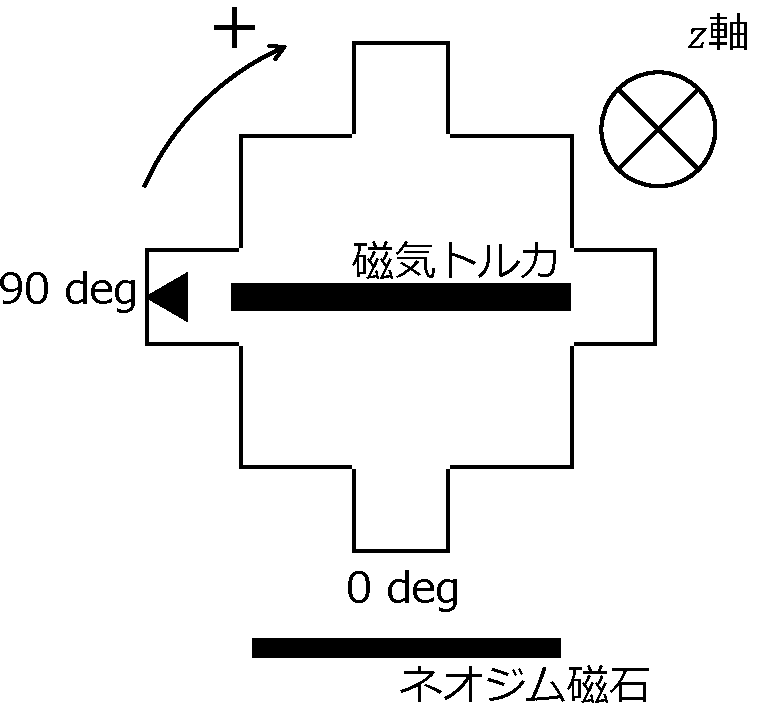
\includegraphics[width=\columnwidth]{./figure/90deg-crop.pdf}
	  \subcaption{角度}
	  \label{fig:90deg}
	\end{minipage}
	\hspace{5mm}
	\begin{minipage}{0.3\columnwidth}
	  \centering
	  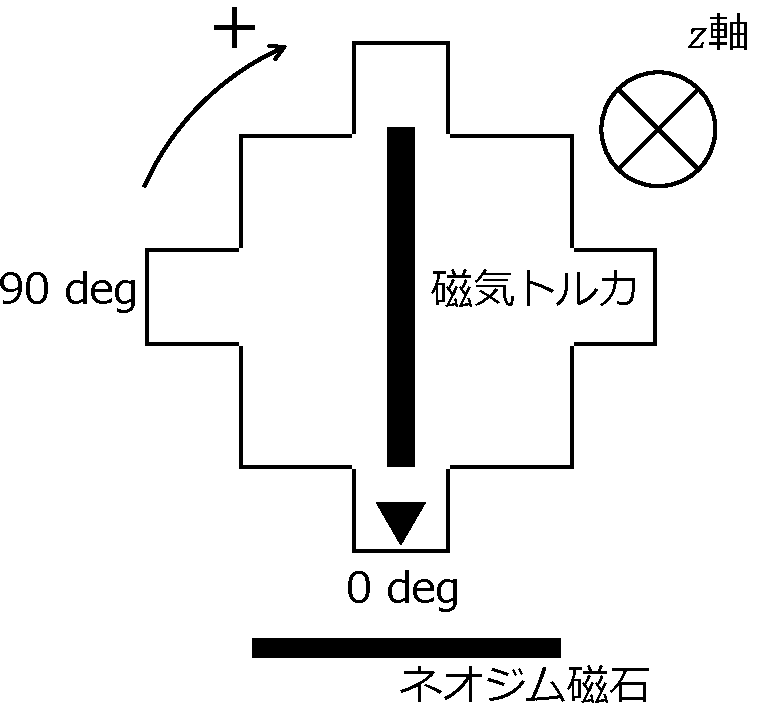
\includegraphics[width=\columnwidth]{./figure/0deg-crop.pdf}
	  \caption{角速度}
	  \label{fig:0deg}
	\end{minipage}
	\caption{Duty比50\%としたとき}
	\label{fig:method}
  \end{figure}

\subsection{Duty比100\%・Duty比50\%による制御}
\subsubsection{実験方法}
 PWM信号のDuty比を,50\%と100\%として実験を行う.


\subsubsection{実験結果}
 Duty比を50\%としたときの結果を図\ref{fig:duty50deg},図\ref{fig:duty50degpers}に,100\%としたときの結果を図\ref{fig:duty100deg},図\ref{fig:duty100degpers}に示す.
図に示すようにオーバーシュートが大きく,振動回数が2回となっている.
また,磁気トルカに触ると明らかに発熱していた.
発熱を抑えようとすれば整定時間が伸びる傾向にあった.

\begin{figure}[h]
	\centering
	\begin{minipage}{0.43\columnwidth}
	  \centering
	  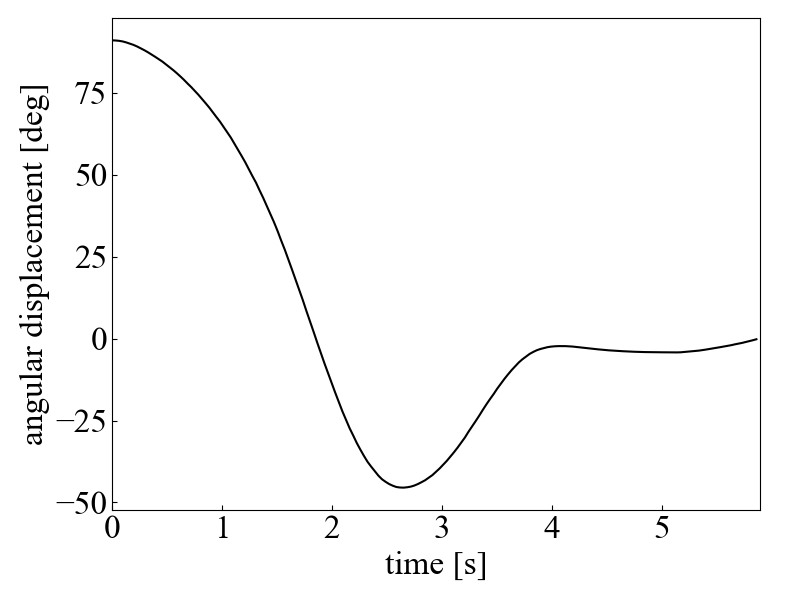
\includegraphics[width=\columnwidth]{./figure/duty50deg.png}
	  \subcaption{角度}
	  \label{fig:duty50deg}
	\end{minipage}
	\hspace{5mm}
	\begin{minipage}{0.43\columnwidth}
	  \centering
	  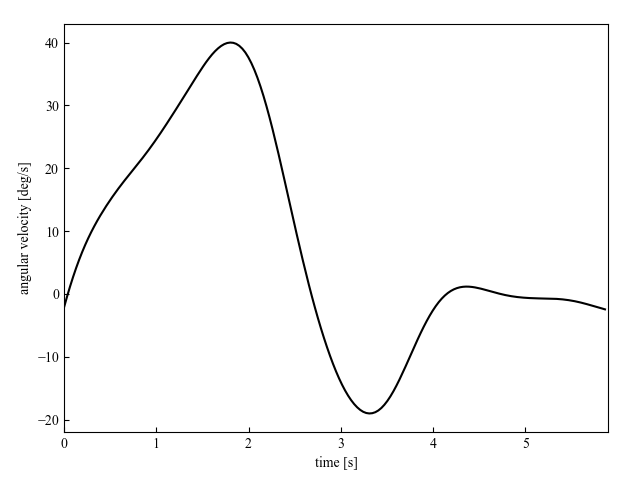
\includegraphics[width=\columnwidth]{./figure/duty50degpers.png}
	  \caption{角速度}
	  \label{fig:duty50degpers}
	\end{minipage}
	\caption{Duty比50\%としたとき}
	\label{fig:Duty50}
  \end{figure}

  \begin{figure}[h]
	\centering
	\begin{minipage}{0.43\columnwidth}
	  \centering
	  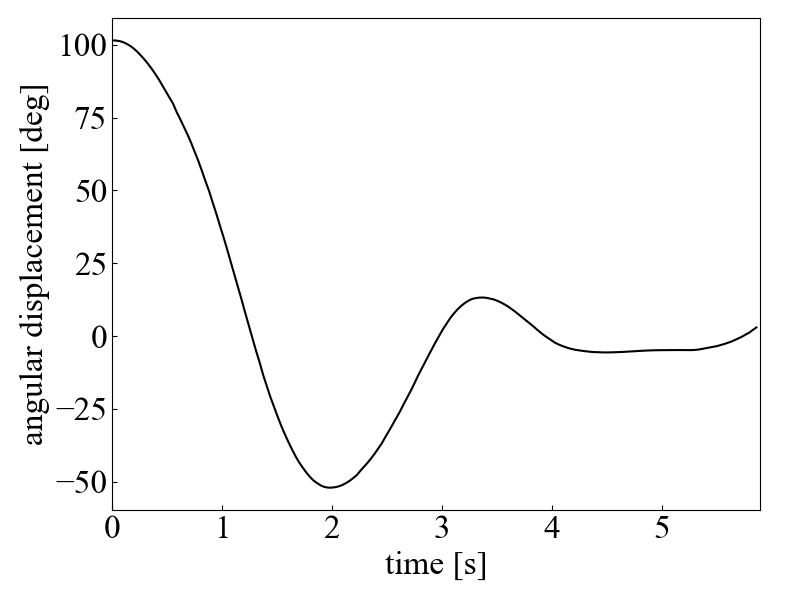
\includegraphics[width=\columnwidth]{./figure/duty100deg.png}
	  \subcaption{角度}
	  \label{fig:duty100deg}
	\end{minipage}
	\hspace{5mm}
	\begin{minipage}{0.43\columnwidth}
	  \centering
	  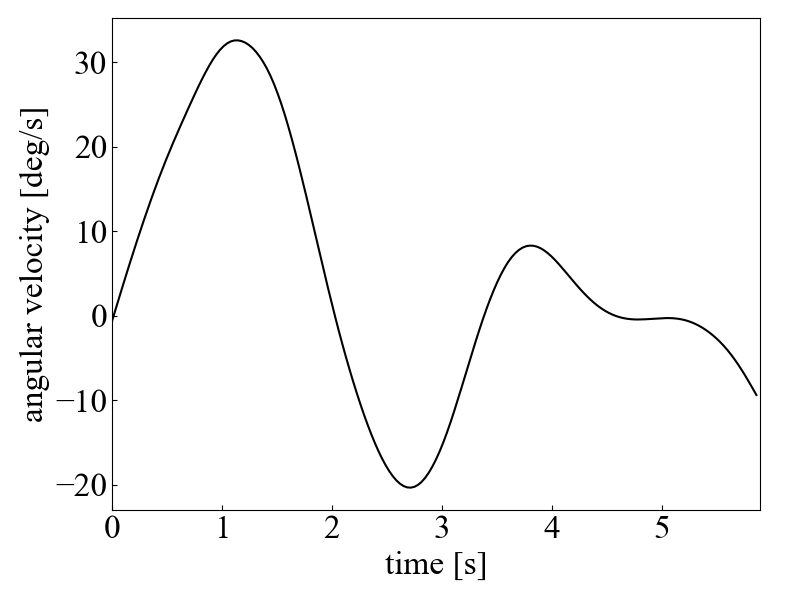
\includegraphics[width=\columnwidth]{./figure/duty100degpers.png}
	  \subcaption{角速度}
	  \label{fig:duty100degpers}
	\end{minipage}
	\caption{Duty比を100\%としたとき}
  \end{figure}

\newpage

\subsection{P制御}
\subsubsection{実験方法}
 Pコントローラを$I(t) = k_P |\theta(t)|$とし,実験を行う.

\subsubsection{実験結果}
 何度か実験を行って$k_P$を調整し,$k_P=0.05$としたときの結果を図\ref{fig:Pdeg},図\ref{fig:Pdegpers}に示す.
整定時間は3.8 s ,定常偏差は2.78 deg であった.

\begin{figure}[h]
	\centering
	\begin{minipage}{0.43\columnwidth}
	  \centering
	  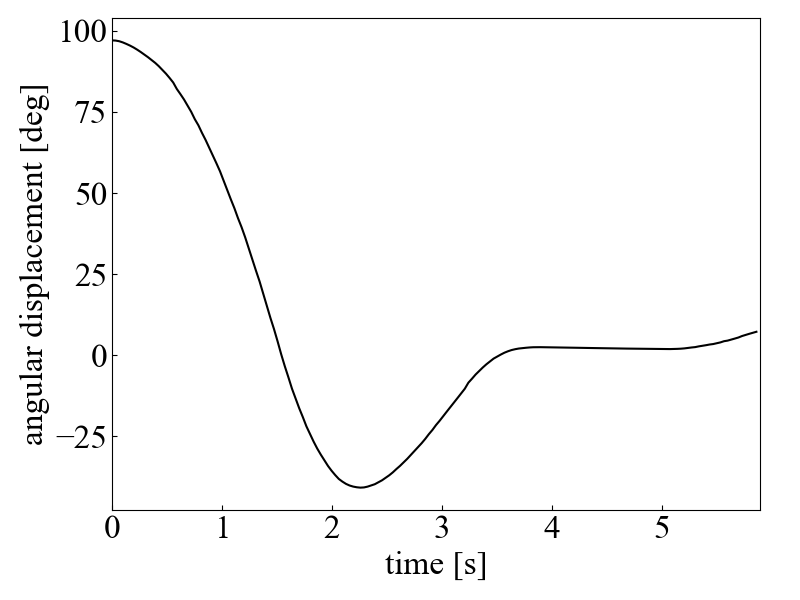
\includegraphics[width=\columnwidth]{./figure/Pdeg.png}
	  \subcaption{角度}
	  \label{fig:Pdeg}
	\end{minipage}
	\hspace{5mm}
	\begin{minipage}{0.43\columnwidth}
	  \centering
	  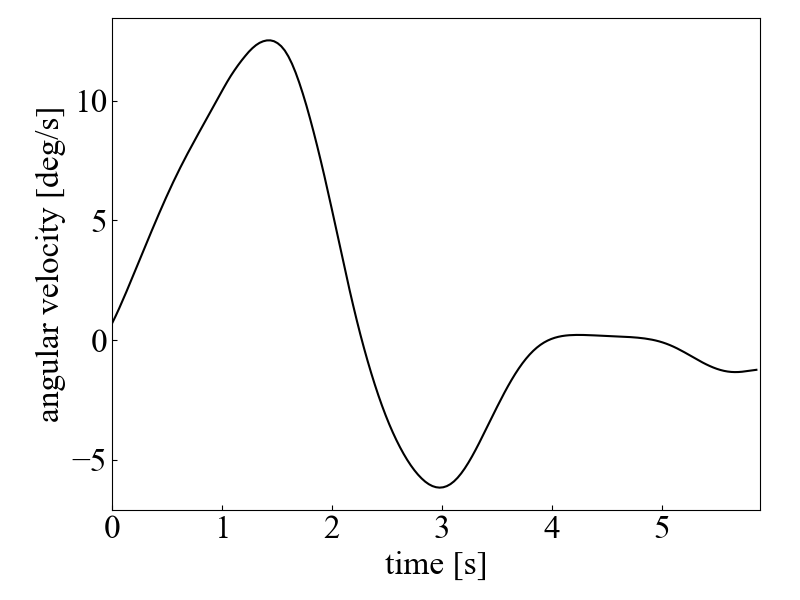
\includegraphics[width=\columnwidth]{./figure/Pdegpers.png}
	  \subcaption{角速度}
	  \label{fig:Pdegpers}
	\end{minipage}
	\caption{P制御}
	\label{fig:P}
  \end{figure}

\newpage

\subsection{PD制御}
\subsubsection{実験方法}
 Pコントローラを$I(t) = k_P |\theta(t)| + k_D|\frac{d\theta(t)}{dt}|$とする.
なお,$\frac{d\theta(t)}{dt}$は,プログラムの1ループ前の角度を$\theta_\mathrm{pre}(t)$とし,$\frac{d\theta(t)}{dt} = \theta(t)-\theta_\mathrm{pre}(t)$で近似する.
\subsubsection{実験結果}
 何度か実験を行ってゲインを調整し,$k_P=0.03$,$k_P=0.05$としたときの結果を図\ref{fig:PDdeg},図\ref{fig:PDdegpers}に示す.
整定時間は4.0 s ,定常偏差は-21.3 deg であった.
\begin{figure}[h]
	\centering
	\begin{minipage}{0.43\columnwidth}
	  \centering
	  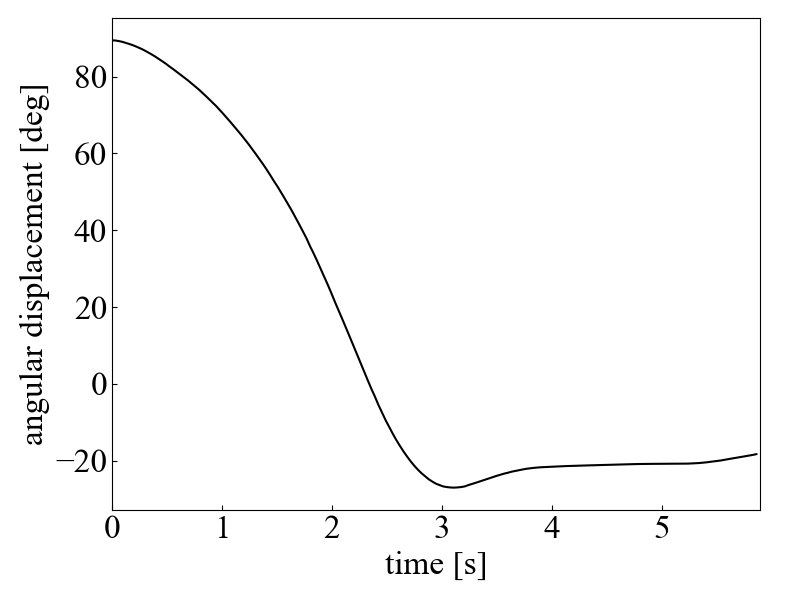
\includegraphics[width=\columnwidth]{./figure/PDdeg.png}
	  \subcaption{角度}
	  \label{fig:PDdeg}
	\end{minipage}
	\hspace{5mm}
	\begin{minipage}{0.43\columnwidth}
	  \centering
	  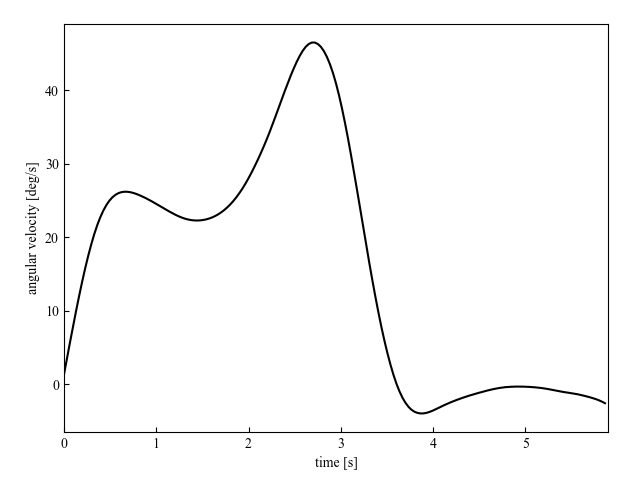
\includegraphics[width=\columnwidth]{./figure/PDdegpers.png}
	  \subcaption{角速度}
	  \label{fig:PDdegpers}
	\end{minipage}
	\caption{PD制御}
	\label{fig:PD}
  \end{figure}

\subsection{B-dot制御則}
\subsubsection{実験方法}
 搭載する磁気トルカが1つであるので,目標磁気モーメントは$M=-k_bB_y\omega_z$である.
$|M|=nIS$より,コントローラを$I=\frac{-k_bB_y\omega_z}{nS}$として実験を行う.

\subsubsection{実験結果}
 $k_b=0.02,k_b=0.05,k_b=0.15$としたときの結果を図\ref{fig:bdotdeg},図\ref{fig:bdotdegpers}に示す.
整定時間は3.0 s ,定常偏差は-13.4 deg であった.

\begin{figure}[h]
	\centering
	\begin{minipage}{0.43\columnwidth}
	  \centering
	  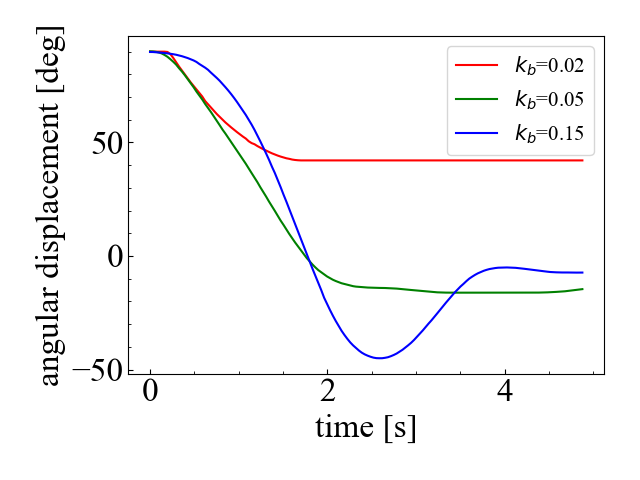
\includegraphics[width=\columnwidth]{./figure/kb5deg.png}
	  \subcaption{角度}
	  \label{fig:bdotdeg}
	\end{minipage}
	\hspace{5mm}
	\begin{minipage}{0.43\columnwidth}
	  \centering
	  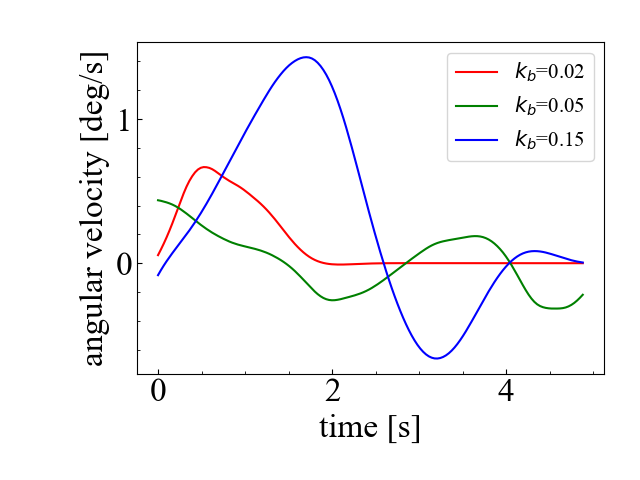
\includegraphics[width=\columnwidth]{./figure/kb5degpers.png}
	  \subcaption{角速度}
	  \label{fig:bdotdegpers}
	\end{minipage}
	\caption{B-dot制御則}
	\label{fig:bdot}
\end{figure}

\newpage

\subsection{クロスプロダクト則}
\subsubsection{実験方法}
 目標磁気モーメントが$M = \frac{K_x c_z + k_x \omega_z}{B_y}$であるので,
コントローラを$I=\frac{K_x c_z + k_x \omega_z}{nSB_y}$として実験を行う.

\subsubsection{実験結果}
 $K_x=0.04$,$k_x=0.03$としたときの結果を図\ref{fig:crossdeg},図\ref{fig:crossdegpers}に示す.
整定時間は3.8 s ,定常偏差は0.1 deg であった.

\begin{figure}[h]
	\centering
	\begin{minipage}{0.43\columnwidth}
	  \centering
	  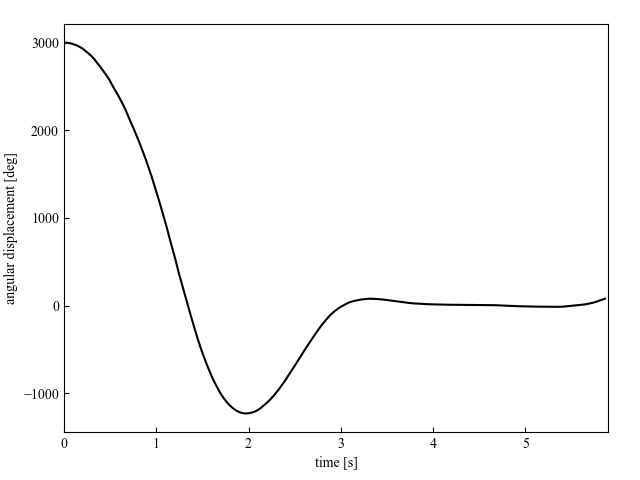
\includegraphics[width=\columnwidth]{./figure/crossdeg.png}
	  \subcaption{角度}
	  \label{fig:crossdeg}
	\end{minipage}
	\hspace{5mm}
	\begin{minipage}{0.43\columnwidth}
	  \centering
	  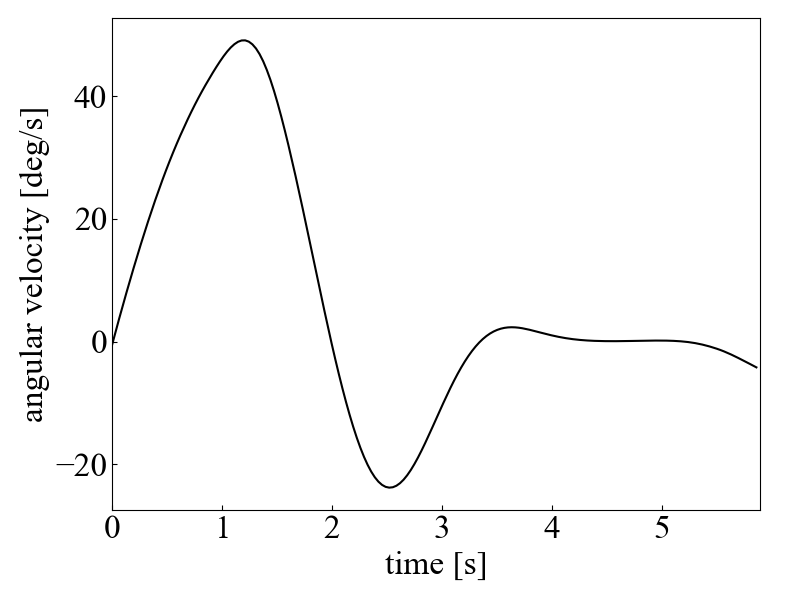
\includegraphics[width=\columnwidth]{./figure/crossdegpers.png}
	  \subcaption{角速度}
	  \label{fig:crossdegpers}
	\end{minipage}
	\caption{クロスプロダクト則}
	\label{fig:cross}
\end{figure}


\subsection{考察}
 各結果の整定時間,定常偏差を表\ref{table:result}に示す.
この表から,整定時間に基づいて評価すればB-dot制御則が最適であり,
定常偏差に基づいて評価すればクロスプロダクト則が最も優れた制御則となる結果を得た.
P,PD,クロスプロダクト則は,制御量が角度であるのに対して積分要素を含まないため,ゲインの組み合わせによっては定常偏差が残る.
B-dot制御則は制御量が角速度であるため,定常偏差が残っている.

\begin{table}[H]
	\centering
	\caption{実験結果}
	\label{table:result}
	\begin{tabular}{|c||c|c|c|c|c|c|}
		\hline
		 & 50\% & 100\% & P制御 & PD制御 & B-dot制御則 & クロスプロダクト制御則 \\ \hline
		整定時間T [s] & 4.1 & 4.3 & 3.8 & 4.0 & 3.0 & 3.8 \\ \hline
		定常偏差$\theta$ [deg] & 0 & 0 & 2.78 & -21.3 & -13.4 & 0.1 \\ \hline
	\end{tabular}
\end{table}


\newpage
\section{結論}
\subsection{本研究のまとめ}
 本研究では,人工衛星の模型や実験システムを新規に作製して,磁気トルカによる姿勢制御を検証した.

B-dot制御則については,制御理論の特徴が現れる結果となった.
しかし,PD制御・クロスプロダクト則についてはゲイン設定の余地があり,

本研究で作製した実験装置は,転がり軸受の摩擦や外部電源との接続といった部分で宇宙空間の環境とは程遠く,


先行研究では,想定される人工衛星の大きさの違いや,磁気トルカでの検証を行われていなかったため,超小型人工衛星の,特に磁気トルカに注目して実験装置を作製し,検証を行った.定常偏差を無視すればB-dot制御則が,定常偏差を考慮すればクロスプロダクト則が最も性能の良い制御理論となる結果を得た.
\subsection{今後の展望}

 摩擦の影響がない宇宙空間を想定すると,積分要素が含まれていなくても定常偏差は残らない.転がり軸受の工夫等により摩擦をさらに軽減できれば,PD制御・クロスプロダクト則は定常偏差が残らず,B-dot制御則との役割の違いが現れ,評価が変わる可能性がある. 

 今回は磁気トルカを1本のみ用いて検証を行った.しかし実際の人工衛星の姿勢制御では,1軸に対して磁気トルカを2本用いて姿勢制御を行っていることも多いため,磁気トルカをもう1本増やした検証も必要であると考える.

また,作製した模型の質量,大きさなどから宇宙空間での挙動のシミュレーションを行い,その結果との類似点・相違点を比較して改良点を考える.